\documentclass[oneside,a4paper,12pt]{article}
\usepackage{graphicx}
\usepackage{amsmath}
\usepackage{listings}
\graphicspath{{~/templates/}, {../images/}}

\makeindex
\begin{document}
	\begin{titlepage}
		\includegraphics[width=4cm]{logopopo.png}
		\hspace*{\fill}
		\includegraphics[width=6cm]{logouniv.png}
		
		\begin{center}
			\vspace{1cm}
			\textbf{TP Support de Transmission}\\
			\textbf{Caractèrisation d'antennes}\\
			\vspace{1cm}
			\textbf{Maxence LAURENT, Thibault VOLLERIN, Maxence NEUS}\\
			\vspace{3cm}
			%\includegraphics[width=13cm]{titlepage.png}\\
			\vspace{\fill}
			\textbf{Mars 2022}\\
		\end{center}
	\end{titlepage}
	
	\tableofcontents
	
	\vspace{5cm}
	
	\begin{abstract}
	Le but de ce TP consiste à caractèriser une antenne cornet pyramidal.
	Plus précisement, nous mesurerons le diagramme de rayonnement de l'antenne dans les plans E et H, ainsi que le gain de l'antenne. 
 	\end{abstract}

	\newpage

	\section{Préparation}
	
	\paragraph{1.} 
	Le plan E est défini par le plan $ (x, z) $, c'est à dire $ \phi = 0 $ et $ \theta \in [0; 2 \pi] $.
	
	\paragraph{2.} 
	Le plan H est défini par le plan $ (y, z) $, c'est à dire $ \phi \in [0; 2 \pi] $ et $ \theta = 0 $.
	
	\paragraph{3.}
	\paragraph{}

	\begin{figure}[h]
		\centering
		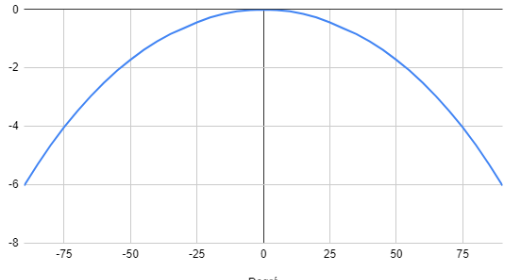
\includegraphics[width=8cm]{prepaPlanE.png}
		\caption{Diagramme de rayonnement dans le plan E}
	\end{figure}

	\begin{figure}[h]
		\centering
		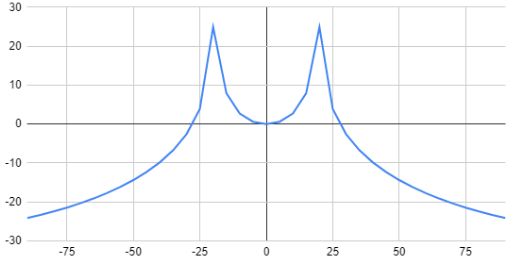
\includegraphics[width=8cm]{prepaPlanH.png}
		\caption{Diagramme de rayonnement dans le plan H}
	\end{figure}

	\paragraph{4.}
	\begin{itemize}
		\item[Plan E] : 65° d'ouverture
		\item[Plan H] : 30° d'ouverture 
	\end{itemize}

	\newpage

	\section{Manipulations}

	\subsection{Etalonage}

	On mesure les pertes du grand cable : $-1.6dB$.
	
	\subsection{Diagramme de rayonnement}

	\paragraph{Plan H}

	\begin{figure}[h]
		\centering
		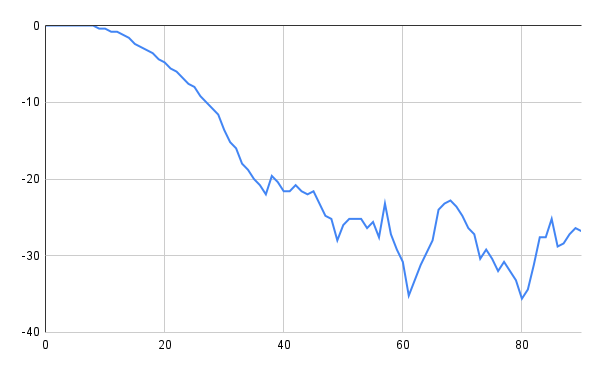
\includegraphics[width=8cm]{planH.png}
		\caption{Puissance reçue dans le plan H}
	\end{figure}

	On lit une chute de 3dB à 17° Soit un angle d'ouverture à 3dB de 34°.

	\paragraph{Plan E}

	\begin{figure}[h]
		\centering
		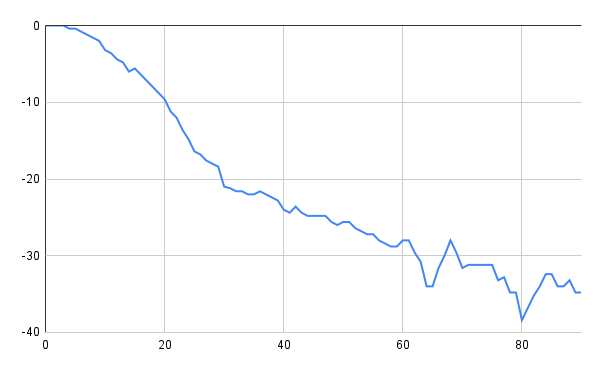
\includegraphics[width=8cm]{planE.png}
		\caption{Puissance reçue dans le plan E}
	\end{figure}

	On lit une chute de 3dB à 12° Soit un angle d'ouverture à 3dB de 24°.

	\subsection{Gain de l'antenne}

	On emet toujours 10dBm avec la première antenne et on va lire la puissance reçue à la seconde.
	On tiendra compte des pertes du long cable de l'antenne à la réception calculées en 2.1

	On donne:
	\[ P_{d} = P_{t}.G_{t}.G_{r}.(\frac{\lambda}{4 \pi R})^{2} \]

	En supposant que les deux antennes sont bien identiques et ont donc le même gain,
	on peut tracer $ \frac{P_{d}}{P_{t}} = f(\frac{1}{R^{2}}) $ et le graph devrait être une droite de pente $ G^{2}*(\frac{\lambda}{4 \pi})^{2} $.
	On réalisera une régression linéaire pour obtenir la valeur de G en connaisant les autres paramètres.

	\begin{figure}[h]
		\centering
		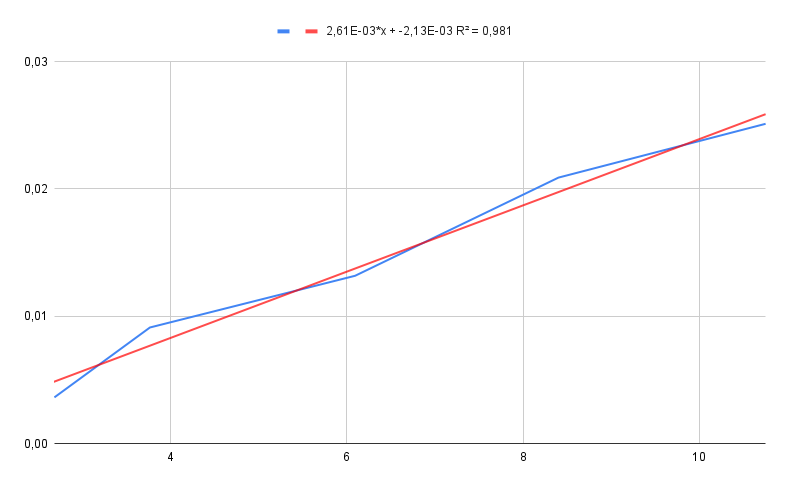
\includegraphics[width=10cm]{gainAntenne.png}
		\caption{Rapport $ \frac{P_{d}}{P_{t}} = f(\frac{1}{R^{2}}) $ }
	\end{figure}

	On obtient une pente à 26,1.
	Donc \[ 2,61e^{-3} = G^{2}*(\frac{\lambda}{4 \pi})^{2} \]
	Et on donne \[ G=17.9 dB \]

	\newpage
	\section{Conclusion}
	Nous avons dans ce TP utilisé les propriétés de symètrie des antennes pour réduire le nombre de mesures nécessaires à la caractèrisation complète du diagramme de rayonnement.
	La caractèrisation de l'antenne est un procédé qui, à la main, prend du temps mais qui est nécessaire à la bonne conception des systèmes.
		

\end{document}
